%% vim: set sts=4 et :

\chapter{Usage}
\label{ch:usage}

\EOS has been authored with several use cases in mind.
\begin{enumerate}
\item The evaluation of observables and further theoretical quantities in the
field of flavor physics. \EOS aspires to produce theory estimates of publication
quality, and has produced such estimates in the past.

\item The inference of parameters from experimental observations.  For this
task, \EOS defaults to the Bayesian framework of parameter inference.

\item The production of toy events for a variety of flavor-physics-related
processes using Monte Carlo methods.
\end{enumerate}

In the remainder of this chapter we document the usage of the existing \EOS
clients and scripts, to carry out tasks corresponding to the above use
cases. We assume further that only the built-in observables, physics models
and experimental constraints are used. The necessary steps to extend EOS with
new observables, physics models or constraints is discussed in \refch{extending}.


\section{Browsing the List of Parameters, Observables and Constraints}
\label{sec:usage:parameters+observables+constraints}

\EOS has understands parameters, observables, options, kinematic variables, and
constraints.  Parameters, observables and constraints share a common naming
scheme, in order to allow categorize these quantities more readily. The naming
scheme is as follows: each name can be decomposed into a prefix (before the
\texttt{::} separator), an optional tag (after the optional \texttt{\@}
separator), and the short name (between the separators); e.g.:
\begin{center}
    \verb+K^*::a_1_para@1GeV+
\end{center}
Here \texttt{K\^{}*} indicated the association with the $K^*$ meson,
\texttt{a\_1\_para} is the short name for this object, and the tag is present and
reads \texttt{1GeV}.\\

Parameters are scalar floating-point-valued inputs. They are real-valued
numbers that can be set to arbitrarily at run time.  The full list of
parameters known to EOS as well as their default values and ranges can be browsed
by running \client{eos-list-parameters}.\\

Observables are \EOS-internal functions that take a set of parameters and return a single
(real-valued) number. These functions take a set of kinematic variables as their arguments.
They include true observables in the physical sense (e.g.
a branching ratio) but also pseudo observables such as hadronic form factors.
A full list of observables known to EOS can be listed by running
\client{eos-list-observables}.\\

Options are used to modify the behaviour of an observable at run time.
Universal examples include changing the physics model (via \option{model}) and
changing form factor parametrisation (via \option{form-factors}). However,
generally their names are specific to a single observable. There is presently
no way to list all possible options that pertain to a given observable.\\

Kinematic variables are used to provide numerical inputs to an observable that can
be changed on a per-observable level. As such, the names of kinematic variables are
specific to each observable. The required kinematic variables for each observable
can be looked up using the \client{eos-list-observables} client.\\

Constraints represent individual likelihood functions, either of
an experimental measurement or a theoretical prediction. The list of built-in
constraints is available through \client{eos-list-constraints}.


\section{Evaluating Observables}
\label{sec:usage:eos-evaluate}

Observables can be evaluated using \client{eos-evaluate}. It accepts
the following command line arguments:
\begin{itemize}
    \item[] \cli{--kinematics NAME VALUE}\\[\medskipamount]
        Within the scope of the next observable, declare a new kinematic
        variable with name \cli{NAME} and numerical value \cli{VALUE}.

    \item[] \cli{--range NAME MIN MAX POINTS}\\[\medskipamount]
        Within the scope of the next observable, declare a new kinematic
        variable with name \cli{NAME}. Subdivide the interval [\cli{MIN}, \cli{MAX}]
        in \cli{POINTS} subintervals, and evaluate the observable at each subinterval
        boundary.\\

        \emph{Note}: More than one \cli{--range} command can be issued per
        observable, but only one \cli{--range} command per kinematic variable.

    \item[] \cli{--observable NAME}\\[\medskipamount]
        Add a new observable with name \cli{NAME} to the list of observables
        that shall be evaluated. All previously issued \cli{--kinematics}
        and \cli{--range} arguments apply, and will be used by the new obervable.
        The kinematics will be reset (i.e., all kinematic variables will be removed)
        in anticipation of the next \cli{--observable} argument.

    \item[] \cli{--vary NAME}\\[\medskipamount]
        Estimate the uncertainty based on variation of the parameter \cli{NAME},
        as if the parameter was distributed like a univariate Gaussian.

    \item[] \cli{--budget NAME}\\[\medskipamount]
        Create a new uncertainty budget, which encompasses all the subsequently issued
        \cli{--vary} commands (until the issue of a new \cli{--budget} command).
        By default, the \texttt{delta} budget always exists, and encompasses \emph{all}
        variations.
\end{itemize}

As an example, we use the evaluation of the $q^2$-integrated branching ratio
$\mathcal{B}(\bar{B}^0\to \pi^+\mu^-\bar\nu_\mu)$, which is addressable as
\observable{B->pilnu::BR}. For this example, we use the integration range
\begin{equation*}
    0\,\GeV^2 \leq q^2 \leq 12\,\GeV^2\,.
\end{equation*}
Further, we use the \option{BCL2008} \cite{Bourrely:2008za} parametrization of the
$\bar{B}\to \pi$ form factor, as well as the Wolfenstein parametrization of the
CKM matrix. The latter is achieved by choosing the physics model \option{SM}. By
default, \EOS uses the most recent results of the UTfit collaboration's fit of
the CKM Wolfenstein parameter to data on tree-level decays.  In this example,
we evaluate the observable and estimate parametric uncertainties based on
the naive expectation of Gaussian uncertainty propagation. We
classify two budgets of parametric uncertainties: one for uncertainties
pertaining to the form factors (labelled 'FF'), and one for uncertainties
pertaining to the CKM matrix elements (labelled 'CKM').

Our intentions translate to the following call to \client{eos-evaluate}:
\commandlineexample{examples/evaluate-btopilnu-integrated.bash}

\begin{filecontents*}{examples/evaluate-btopilnu-integrated.out}
# B->pilnu::BR: form-factors=BCL2008,l=mu
# s_min	s_max	central	FF_min	FF_max	CKM_min	CKM_max	delta_min	delta_max
0	12	0.000106816	3.00927e-05	1.46426e-05	9.14007e-06	9.70515e-06	3.14501e-05	1.75669e-05   (-29.4434% / +16.446%)
\end{filecontents*}
The above call yields the following output:
\commandlineexample{examples/evaluate-btopilnu-integrated.out}

The output of calls to \client{eos-evaluate} is structured as follows:
\begin{itemize}
    \item The first row names the observable at hand, as well as all active options.
    \item The second row contains column headers in the order:
        \begin{itemize}
            \item kinematics variables,
            \item the upper and lower uncertainty estimates for each individual uncertainty budget,
            \item the total upper and lower uncertainty estimates.
        \end{itemize}
    \item The third row contains the result as described by the above columns. In addition, at
        the end of the row the relative total uncertainties are given in parantheses.
\end{itemize}
The above structure repeats itself for every observable, as well as for each variation point
of the kinematic variables as described by occuring \cli{--range} arguments.\\

\section{Producing Random Parameter Samples}
\label{sec:usage:eos-sample-mcmc+pmc}

For all the previously mentioned use cases (observable evaluation, Bayesian
parameter inference, and production of pseudo events) one requires to draw
random samples from some arbitrary \gls{PDF} $P(\vec\theta)$.  When using \EOS,
these random samples can be produced from \gls{MCMC} random walks, using the
Metropolis-Hastings algorithm, by calls to the \client{eos-sample-mcmc} client.
In a second step, refined samples or samples for a very complicated setup, can
be obtained from an algorithm described in Ref.~\cite{Beaujean:2013}. This
algorithm uses an adaptive importance sampling called Population Monte Carlo
(PMC), implemented within the client \client{eos-sample-pmc}, and requires a
prior run of \client{eos-sample-mcmc} for initialization.\\


The follow command-line arguments are common to the \client{eos-sample-mcmc} and 
\client{eos-sample-pmc} clients, as well as further clients described in subsequent
sections:
\begin{itemize}
    \item[] \cli{--scan NAME --prior flat MIN MAX}\\[-3\medskipamount]
    \item[] \cli{--scan NAME [ABSMIN ABSMAX] --prior gaussian MIN CENTRAL MAX}\\[-3\medskipamount]
    \item[] \cli{--nuisance [...]}\\[\medskipamount]
        These arguments add a parameter to the statistical analysis, with
        either a flat or a gaussian prior. If \cli{ABSMIN} and
        \cli{ABSMAX} are specified, the prior will be cropped to this
        absolute interval.  The \cli{--scan} and \cli{--nuisance}
        arguments work identically, with one exception: \cli{--nuisance}
        declares the associated parameter as a nuisance parameter, which is
        flagged in the \gls{HDF5} output. The sampling algorithm treats nuisance
        parameters \emph{in the same way as} scan parameters.

    \item[] \cli{--constraint NAME}\\[\medskipamount]
        The named constraint from the internal database will be used as part of
        the likelihood. The functional form of the the likelihood, details such
        as correlations, and the required options for the observables used will
        be automatically looked up. In order to browse the entries of the
        database, use the \client{eos-list-constraints} client.

    \item[] \cli{--fix NAME VALUE}\\[\medskipamount]
        The value of parameter \cli{NAME} will be set to the supplied
        \cli{VALUE}, and thus potentially deviate from its default value.
\end{itemize}

The \client{eos-sample-mcmc} client further accepts the following arguments:
\begin{itemize}
    \item[] \cli{--seed [time|VALUE]}\\[\medskipamount]
        This argument sets the seed value for the \gls{RNG}. Setting the
        seed to a fixed numerical \cli{VALUE} ensures reproducibility of the results. This
        is important for publication-quality usage of the client. If \cli{time} is
        specified, the \gls{RNG} is seeded with an interger value based on the current time.

    \item[] \cli{--prerun-min VALUE}\\[\medskipamount]
        For the prerun phase of the sampling algorithm, set the minimum number of
        steps to \cli{VALUE}.

    \item[] \cli{--prerun-max VALUE}\\[\medskipamount]
        For the prerun phase of the sampling algorithm, set the maximum number of
        steps to \cli{VALUE}.

    \item[] \cli{--prerun-update VALUE}\\[\medskipamount]
        For the prerun phase of the sampling algorithm, force an adaptation of the
        Markov chain's proposal function to its environment after every \cli{VALUE}
        steps.

    \item[] \cli{--store-prerun [0|1]}\\[\medskipamount]
        Either disable or enable storing of the prerun samples to the output file.\\

    \item[] \cli{--output FILENAME}\\[\medskipamount]
        Use the file \cli{FILENAME} to store the output, using the \gls{HDF5} file format.
        The resulting \gls{HDF5} file follows the EOS-\gls{MCMC} format, and can be accessed using, e.g.,
        the \texttt{eosdata} Python module.
\end{itemize}

The \client{eos-sample-pmc} client additionally accepts the following command-line arguments:
\begin{itemize}
    \item[] \cli{--seed [time|VALUE]}\\[\medskipamount]
        This argument sets the seed value for the \gls{RNG}. Setting the
        seed to a fixed numerical \cli{VALUE} ensures reproducibility of the results. This
        is important for publication-quality usage of the client. If \cli{time} is
        specified, the \gls{RNG} is seeded with an interger value based on the current time.

    \item[] \cli{--hc-target-ncomponents N}\\[\medskipamount]
        When creating mixture components, create \cli{N} components per existing
        MC group.

    \item[] \cli{--hc-patch-length LENGTH}\\[\medskipamount]
        When clustering a group's MCs onto the mixture components, cut the
        chains into patches of \cli{LENGTH} samples each.

    \item[] \cli{--hc-skip-initial FRACTION}\\[\medskipamount]
        Skip the first \cli{FRACTION} of all MCMC samples in the clustering step.

        \emph{Note}: \cli{FRACTION} must be a decimal number between $0$ and $1$.

    \item[] \cli{--pmc-initialize-from-file HDF5FILE}\\[\medskipamount]
        Use the samples from a MCMC HDF5 output file \cli{HDF5FILE} as
        generated with \client{eos-sample-mcmc}, in order to initialize the
        mixture density of the initial PMC step.

    \item[] \cli{--pmc-group-by-r-value R}\\[\medskipamount]
        When forming groups of MCs from the initialization file, only add
        a chain to an existing group if the chain's $R$-value is less than \cli{R};
        create a new group otherwise.

    \item[] \cli{--pmc-samples-per-component N}\\[\medskipamount]
        Set the number \cli{N} of samples that will be drawn per component and
        per update step of the PMC run.

    \item[] \cli{--pmc-final-samples N}\\[\medskipamount]
        Set the number \cli{N} of samples that will be drawn for the final step,
        i.e.: after the PMC updates have converged.

    \item[] \cli{--pmc-relative-std-deviation-over-last-step STD STEPS}\\[\medskipamount]
        If both perplexity and ESS have a standard deviation less than \cli{STD} over the
        last \cli{STEPS} updates, declare convergence.

    \item[] \cli{--pmc-ignore-ess [0|1]}\\[\medskipamount]
        Set whether convergence of the PMC updates shall be determined from the
        effective sample size (ESS) \emph{in addition} to the perplexity.\\
        \emph{Default}: Use the ESS.

    \item[] \cli{--output FILENAME}\\[\medskipamount]
        Use the file \cli{FILENAME} to store the output, using the \gls{HDF5}
        file format.  The resulting \gls{HDF5} file follows the EOS-\gls{PMC}
        structure, and can be read using the \texttt{eosdata} Python
        module.
\end{itemize}

As an example, we define the a-priori \gls{PDF} for a study of the decay $\bar{B}\to \pi^+\mu^-\bar\nu_\mu$.
For the CKM Wolfenstein parameters, we use
\begin{equation*}
\begin{aligned}
    \lambda    & = 0.22535 \pm 0.00065\,,  &
    A          & = 0.807 \pm 0.020\,,      \\
    \bar{\rho} & = 0.128 \pm 0.055\,,      &
    \bar{\eta} & = 0.375 \pm 0.060\,.
\end{aligned}
\end{equation*}
For the a-priori \gls{PDF}, we use uniform distributions for the BCL2008
\cite{Bourrely:2008za} parameters for the $B\to \pi$ form factor $f^{B\pi}_+$.
However, we construct a likelihood from the results of a recent study
(IKMvD2016 \cite{Imsong:2014oqa}) of the form factor $f^{B\pi}_+(q^2)$ within \glspl{LCSR}.
We now intend to draw random numbers from the posterior PDF using EOS' adaptive
Metropolis-Hasting algorithm.  During its prerun phase, the algorithm adapts
the chains' proposal functions. As a consequence, the prerun samples will in
general \emph{not} be distributed as the posterior \gls{PDF}. With a subequent
PMC sampling run in mind, we should demand at least $500$ steps, and -- for a
problem of this complexity -- maximally $7500$ steps during the prerun phase;
the adaption process should be executed after every $500$ steps.\\

Our intentions translate to the following call to \client{eos-sample-mcmc}:
\commandlineexample{examples/sample-mcmc-btopi-ff.bash}

Optionally, if the prerun converges, the client can be used to perform a main run, in which
the proposal functions will be kept static. For such these main run samples, we wish for a
total of $10^4$, which we artifically decompose
into $10$ chunks with $1000$ samples each. While the sampling at hand will be quite quick,
sampling of computationally expensive functions should be done with small chunks so that
the progress of the computations can be monitored. The require options for these intentation
are shown above with a leading hash mark. Also, for a main run,
the \texttt{--prerun-only} flag would need to be removed.\\

We use the above call to \client{eos-sample-mcmc} in order to initialize a PMC
run. We wish for $4$ mixture components per MC group, and to skip $20\%$ of the
MCMC samples as part of the burn in. MC groups will be created based on an
$R$-value \cite{Gelman:1992zz} threshold of $1.5$. For each update, $500$
samples per mixture component shall be drawn, in order to produce $10^6$
samples in the final step. Convergence shall be declared upon a standard
deviation for the perplexity only, of $0.05$ over the last $4$ update steps.
The call then reads: \commandlineexample{examples/sample-pmc-btopi-ff.bash}

Both clients output copious amounts diagnostic data to the standard output, which include
\begin{itemize}
    \item all information about the prior and the likelihood as specified on the command line (both clients);
    \item information about the convergence of the Markov chains within the parameter space,
    based on the $R$-value criterion \cite{Gelman:1992zz} (MCMC only);
    \item information about the convergence of the PMC run based on the perplexity and
    effective sampling size (PMC only).
\end{itemize}

\begin{figure}
    \subfigure[%
        Histogram of the marginal posterior of $|V_{ub}|$, using $4 \times 7500$ samples.
        Despite the poor quality of these samples, they can be used to initialize the
        PMC run as described in the text.
    ]{%
        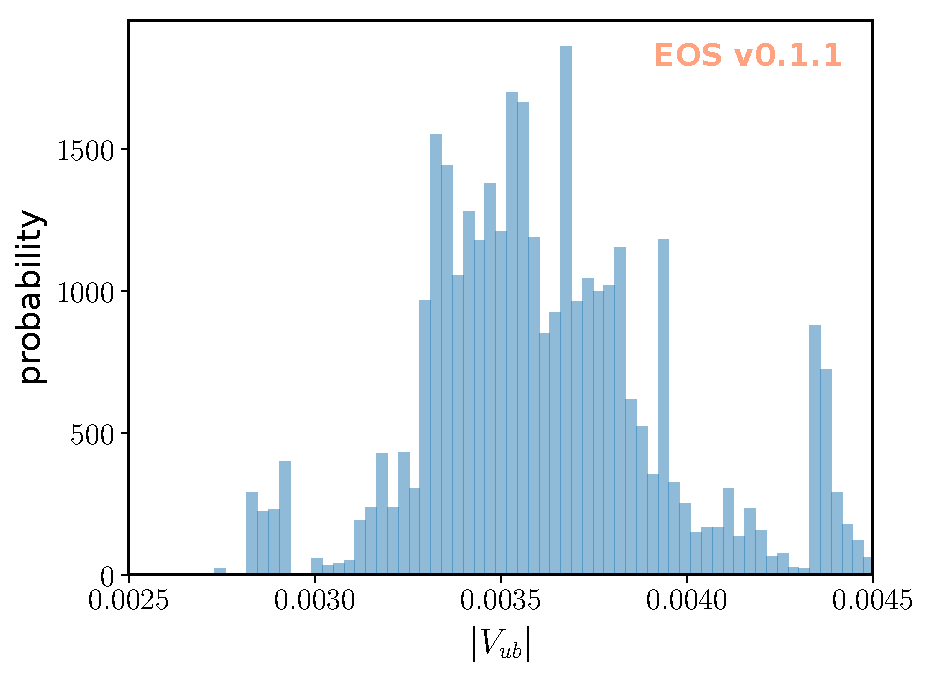
\includegraphics[width=.49\textwidth]{figures/fig-vub-prerun.pdf}
    }\quad
    \subfigure[%
        Histogram of the marginal posterior of $|V_{ub}|$, using $10^6$ samples.
    ]{%
        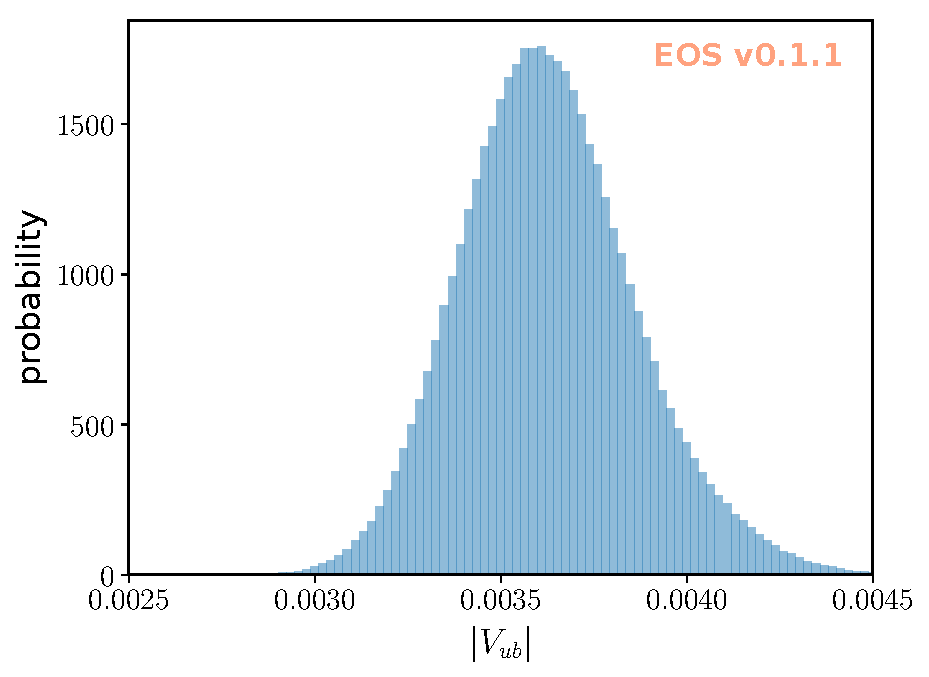
\includegraphics[width=.49\textwidth]{figures/fig-vub-pmc.pdf}
    }
    \caption{%
        Histograms of the parameter of interest $|V_{ub}|$ in the two example
        fits as described in \refsec{usage:eos-sample-mcmc+pmc}, and plotted
        using the \client{eos-plot-1d} client; see \refsec{usage:eos-plot} for
        details.
    }
    \label{fig:usage:vub-example-samples}
\end{figure}

We display the outcome of both the MCMC (prerun) sampling as well as the PMC sampling steps
in \reffig{usage:vub-example-samples}.

\section{Finding the Mode of a Probability Density}
\label{sec:usage:eos-find-mode}

The mode, best-fit point, or simply the most-likely value of some \gls{PDF}
$P(\vec\theta)$ is regularly searched for in physics analyses. EOS supplies the
client \client{eos-find-mode}, which accepts the common set of arguments
describing the PDF as already discussed for the \client{eos-sample-mcmc} and
\client{eos-sample-pmc} clients, see \refsec{usage:eos-sample-mcmc+pmc} for
further information.  In addition, it accepts the following command-line
arguments:
\begin{itemize}
    \item[] \cli{--starting-point \{ VALUE1 VALUE2 ... VALUEN \}}\\[\medskipamount]
        Set the starting point for the maximization of the PDF $P(\vec\theta)$
        at $\theta = ( \cli{VALUE1}, \dots, \cli{VALUEN} )$.
    \item[] \cli{--max-iterations INTEGER}\\[\medskipamount]
        The optimization algorithm is allowed to run at maximum \cli{NUMBER} iterations.
    \item[] \cli{--target-precision NUMBER}\\[\medskipamount]
        Attempt to determine the mode up to an uncertainty of \cli{NUMBER}.
    \item[] \cli{--output FILENAME}\\[\medskipamount]
        Write a YAML file with name \cli{FILENAME} that contains the information of
        the mode in a machine-readable format.
\end{itemize}

In order to illustrate the client's usage, we use the same example as
discussed in \refsec{usage:eos-sample-mcmc+pmc}. The corresponding call
then reads:
\commandlineexample{examples/find-mode-btopi-ff.bash}

\begin{filecontents*}{examples/find-mode-btopi-ff.out}
# Starting optimization at ( 0.0035 0.31 0 0 )

# Found maximum at: 
#   ( 3.568778e-03 2.661032e-01 -2.670912e+00 2.231637e-02 )
#   value = -3.101594e+02
\end{filecontents*}
The output starts with same diagnostic information on the composition of
prior and likelihood as for the sampling clients. The results are displayed
in the last few lines, including
\begin{itemize}
    \item the starting point for the mode-finding process;
    \item the coordinates of the best-fit point; and
    \item the log-posterior at the best-fit point.
\end{itemize}
\commandlineexample{examples/find-mode-btopi-ff.out}

\section{Bayesian Uncertainty Propagation}
\label{sec:usage:eos-propagate-uncertainty}

EOS presently supports two ways to prograpate theory uncertainties in the
framework of Bayesian statistic: First, by using prior PDF that describes
the nuisance parameters; second, by using samples from a posterior PDF that
have been obtained from running \client{eos-sample-pmc}.\footnote{%
    Note that using samples from \client{eos-sample-mcmc} is presently not supported.
}
It accepts the following command-line arguments:
\begin{itemize}
    \item[] \cli{--vary NAME --prior flat MIN MAX}\\[-3\medskipamount]
    \item[] \cli{--vary NAME [ABSMIN ABSMAX] --prior gaussian MIN CENTRAL MAX}\\[\medskipamount]
        These arguments add a parameter to the statistical analysis, with
        either a flat or a gaussian prior. If \cli{ABSMIN} and
        \cli{ABSMAX} are specified, the prior will be cropped to this
        absolute interval.

    \item[] \cli{--samples NUMBER}\\[\medskipamount]
        Sets the number of samples that shall be produced per observable and
        worker thread.

    \item[] \cli{--workers NUMBER}\\[\medskipamount]
        Sets the number of worker threads.

    \item[] \cli{--pmc-input HDF5FILE BEGIN END}\\[\medskipamount]
        Use the samples at index \cli{BEGIN} up to index \cli{END} from
        a named data set in the file \cli{HDF5FILE}.

        \emph{Note:} The file must have been produced by the
        \client{eos-sample-pmc} client.
    \item[] \cli{--pmc-sample-directory NAME}\\[\medskipamount]
        Use the named data set within the file specified with \cli{--pmc-input}.
        Valid names are \texttt{/data/X}, where \text{X} stands for either
        \texttt{initial}, \texttt{final}, or all numbers describing existing
        update steps that were carried out in the PMC run.

        \emph{Note:} You should use \texttt{/data/final} unless you are
        debuging the PMC algorithm.
\end{itemize}

As an example of the first way, we would like to predict the branching
ratio for the decay $B^- \to \tau^- \bar{\nu}_\tau$. This prediction involves
two parameters: First, the absolute value of $V_{ub}$; and second, the value
of the $B$-meson decay constant $f_{B}$. For the former, we choose the
HFAG average of the inclusive determination $|V_{ub}| = (4.45 \pm 0.26) \cdot 10^{-3}$
\cite{Amhis:2014hma}, while for the latter we use the FLAG average
$f_{B} = 0.188 \pm 0.007\,\GeV$ \cite{Aoki:2013ldr}.
Our intention translates to the following call to \client{eos-propagate-uncertainty}:
\commandlineexample{examples/propagate-uncertainty-btotaunu.bash}

As an exmple of the second way, we would like to use samples from the posterior
PDF as obtained in \refsec{usage:eos-sample-mcmc+pmc} in order to predict the
branching ratio of the differential decay $\bar{B}^0\to \pi e^- \bar{\nu}_e$, at various
points in the kinematic range as the decay to muons described previously.
Our intention translates to the following call to \client{eos-propagate-uncertainty}:
\commandlineexample{examples/propagate-uncertainty-btopilnu.bash}

For both ways, the samples of the predictive distributions within the HDF5 files
can be accessed using the \texttt{eosdata} Python module.

\section{Plotting Random Samples}
\label{sec:usage:eos-plot}

Once random samples have been obtained from either a posterior PDF (e.g. as
described in \refsec{usage:eos-sample-mcmc+pmc}) or a predictive PDF (e.g. as
described in \refsec{usage:eos-propagate-uncertainty}), a visual inspection of
the samples is the next step.  EOS provides scripts for this purpose, which
plot histograms of either a marginalized 1D (\client{eos-plot-1d}) or heatmaps
of 2D (\client{eos-plot-2d}) PDFs.  Both scripts presently detect the output
format by inspection of the resepective HDF5 file name. Files containing MCMC
samples should be prefixed with \texttt{mcmc\_}, while PMC sample files should
be prefixed with \texttt{pmc\_monolithic\_}. Files containing samples from the
uncertainty propagation should be prefixed with \texttt{unc\_}.

The \client{eos-plot-1d} produces a 1D histogram of the samples for one parameter.
It accepts the following arguments:
\begin{itemize}
    \item[] \cli{HDF5FILE}\\[\medskipamount]
        The name of the HDF5 input file whose samples shall be plotted.

    \item[] \cli{VAR}\\[\medskipamount]
        The name of the variable (either a \texttt{Parameter} or an \texttt{Observable}) whose
        density function shall be plotted.

    \item[] \cli{PDFFILE}\\[\medskipamount]
        The name of the PDF output file, into which the plot shall be saved.

    \item[] \cli{--xmin XMIN}, \cli{--xmax XMAX}\\[\medskipamount]
        When specified, limit the plot range to the interval \cli{XMIN} to \cli{XMAX}.
        The default values are taken from the description of the parameter within the
        HDF5 input file.

    \item[] \cli{--kde [0|1]}\\[\medskipamount]
        When enabled, plots a univariate Kernel Density Estimate of the probability
        density based on the available samples.

    \item[] \cli{--kde-bandwidth KDEBANDWIDTH}\\[\medskipamount]
        When specified, multiplies the automatically determined KDE bandwidth parameter
        with \cli{KDEBANDWIDTH}.
\end{itemize}

The \client{eos-plot-2d} produces a 2D heatmap of the samples for two parameters.
It accepts the following arguments
\begin{itemize}
    \item[] \cli{HDF5FILE}\\[\medskipamount]
        The name of the HDF5 input file whose samples shall be plotted.

    \item[] \cli{XIDX}\\[\medskipamount]
        The numerical index for the parameter that shall be plotted on the
        $x$ acis. \cli{XIDX} starts with zero

    \item[] \cli{YIDX}\\[\medskipamount]
        The numerical index for the parameter that shall be plotted on the
        $y$ acis. \cli{YIDX} starts with zero

    \item[] \cli{PDFFILE}\\[\medskipamount]
        The name of the PDF output file, into which the plot shall be saved.

    \item[] \cli{--xmin XMIN}, \cli{--xmax XMAX}\\[\medskipamount]
        When specified, limit the plot range on the $x$ axis to the interval
        \cli{XMIN} to \cli{XMAX}. The default values are taken from the
        description of the parameter within the HDF5 input file.

    \item[] \cli{--ymin YMIN}, \cli{--ymax YMAX}\\[\medskipamount]
        When specified, limit the plot range on the $y$ axis to the interval
        \cli{YMIN} to \cli{YMAX}. The default values are taken from the
        description of the parameter within the HDF5 input file.
\end{itemize}
